\documentclass[12pt]{article}
\usepackage[utf8]{inputenc}
\usepackage{float}
\usepackage{amsmath}
\usepackage{graphicx}

\usepackage[hmargin=3cm,vmargin=6.0cm]{geometry}
\topmargin=-2cm
\addtolength{\textheight}{6.5cm}
\addtolength{\textwidth}{2.0cm}
\setlength{\oddsidemargin}{0.0cm}
\setlength{\evensidemargin}{0.0cm}
\usepackage{indentfirst}
\usepackage{amsfonts}

\begin{document}

\section*{Student Information}

Name : Mustafa Alperen Bitirgen \\

ID : 2231496\\


\section*{Answer 1}
\hspace*{-0.6cm}\text{Before we even begin solving the questions, it is safe to first state our groups and related para-}\\
\text{meters in a more formal way so that it gets easier to follow along.}\\
\vspace*{0.2cm}\\
\text{Our first group, X, is people with age 40 and above:}\\
\hspace*{0.6cm}\text{The number of people in this group is 19, such that n$_X$ = 19,}\\
\hspace*{0.6cm}\text{The mean of the answers of this group is 3.375, such that $\bar{X}$ = 3.375,}\\
\hspace*{0.6cm}\text{The standard deviation of the answers of this group is 0.96, such that s$_{X}$ = 0.96.}\\
\vspace*{0.1cm}\\
\text{Our first group, Y, is people with age under 40:}\\
\hspace*{0.6cm}\text{The number of people in this group is 15, such that n$_Y$ = 15,}\\
\hspace*{0.6cm}\text{The mean of the answers of this group is 2.05, such that $\bar{Y}$ = 2.05,}\\
\hspace*{0.6cm}\text{The standard deviation of the answers of this group is 1.12, such that s$_{Y}$ = 1.12.}\\
\vspace*{0.1cm}\\
\text{While we are looking to T table, with degrees of freedom \textit{v} and confidence interval (1-$\alpha$)100\%,}\\
\text{we will use the following representation: T$_{(\textit{v},\alpha)}$. For part \textbf{(a)} and \textbf{(b)} we will need to use the}\\
\text{\textit{Satterthwaite approximation} to approximate the degree of freedom since we have unequal vari-}\\
\text{ances.}\\
\[\textit{v} = \frac{(\frac{s_X^2}{n_X}+\frac{s_Y^2}{n_Y})^2}{\frac{s_X^4}{n_X^2(n_X - 1)} + \frac{s_Y^4}{n_Y^2(n_Y - 1)}}\]\\
\[\hspace*{1.9cm} = \frac{(\frac{0.96^2}{19}+\frac{1.12^2}{15})^2}{\frac{0.96^4}{19^2(19 - 1)} + \frac{1.12^4}{15^2(15 - 1)}} = 27.702\]\\
\text{We have found a non-integer value for \textit{v}. To use the T-table we just take the closest \textit{v} that is}\\
\text{given in that table, which in this case 28.}\\
\subsection*{a)}
\hspace*{-0.6cm}\text{Since we are dealing with means, particularly differences in means, we are going to use T inter-}\\
\text{vals. We are asked to use 95\% confidence interval which corresponds to $\alpha$ = 0.05 but since this }\\
\text{is a two-tailed probability we will use $\frac{\alpha}{2}$ = 0.025 and we have found the degrees of freedom in}\\
\text{solution definition part such that \textit{v} = 28. Our confidence interval will have the form:}\\
\[(\bar{X} - \bar{Y}) \pm T_{(28,0.025)}\sqrt{\frac{s_{X}^2}{n_X} + \frac{s_{Y}^2}{n_Y}}\]\\
\[(3.375 - 2.050) \pm (2.048)\sqrt{\frac{0.96^2}{19} + \frac{1.12^2}{15}}\]\\
\[(1.325) \pm (2.048)\sqrt{\frac{0.9216}{19} + \frac{1.2544}{15}}\]\\
\[(1.325) \pm (2.048)\sqrt{0.1322}\]\\
\[(1.325) \pm (2.048)(0.3635)\]\\
\[1.325 \pm 0.7445 = [0.5805,2.0695]\]\\
\subsection*{b)}
\hspace*{-0.6cm}\text{Since we are dealing with means, particularly differences in means, we are going to use T inter-}\\
\text{vals. We are asked to use 90\% confidence interval which corresponds to $\alpha$ = 0.10 but since this }\\
\text{is a two-tailed probability we will use $\frac{\alpha}{2}$ = 0.05 and we have found the degrees of freedom in}\\
\text{solution definition part such that \textit{v} = 28. Our confidence interval will have the form:}\\
\[(\bar{X} - \bar{Y}) \pm T_{(28,0.05)}\sqrt{\frac{s_{X}^2}{n_X} + \frac{s_{Y}^2}{n_Y}}\]\\
\[(3.375 - 2.050) \pm (1.701)\sqrt{\frac{0.96^2}{19} + \frac{1.12^2}{15}}\]\\
\[(1.325) \pm (1.701)\sqrt{\frac{0.9216}{19} + \frac{1.2544}{15}}\]\\
\[(1.325) \pm (1.701)\sqrt{0.1322}\]\\
\[(1.325) \pm (1.701)(0.3635)\]\\
\[1.325 \pm 0.6183 = [0.7067,1.9433]\]\\
\subsection*{c)}
\hspace*{-0.6cm}\text{Based on the information provided, the significance level is $\alpha$ = 0.05, and the critical value for a}\\
\text{right-tailed test is t$_c$ = 1.734. The rejection region for this left-tailed test is \textbf{\textit{R}} = [ 1.734 , $\infty$)}\\
\text{The t-statistic is computed as follows:}\\
\[\textit{t} = \frac{\bar{X} - 3}{\frac{s_X}{\sqrt{n_X}}}\]\\
\[\hspace*{2.4cm} = \frac{3.375 - 3}{\frac{0.96}{\sqrt{19}}} = 1.703\]\\
\text{Since it is observed that \textit{t} = 1.703 $\leq$ t$_c$ = 1.734, it is then concluded that, we \textbf{can} say people with}\\
\text{age 40 and above supports BREXIT with 95\% confidence level.}\\
\vspace*{0.2cm}\\
\section*{Answer 2}
\hspace*{-0.6cm}\text{Before we even begin solving the questions, it is safe to first state our group and related para-}\\
\text{meters in a more formal way so that it gets easier to follow along.}\\
\vspace*{0.2cm}\\
\[\mu_0 = 20.00;\text{     } \bar{X} = 20.07;\text{    } s_X = 0.07;\text{    } n_X = 11\]\\

\subsection*{a)}
\[H_0: \mu = \mu_0\]\\
\subsection*{b)}
\[H_A: \mu \neq \mu_0\]\\
\subsection*{c)}
\hspace*{-0.6cm}\text{Let us test}\\
\[H_0: \mu = \mu_0 \hspace{0.8cm}\text{ vs }\hspace{0.8cm}H_A: \mu \neq \mu_0\]\\
\text{at a significance level $\alpha$ = 0.01. This corresponds to a two-tailed test, then we will need to take}\\
\text{$\frac{\alpha}{2}$ = 0.005. We have sample statistics:}\\
\[\bar{X} = 20.07 \text{ and, }s_X = 0.07\]\\
\text{Compute the T-statistic,}\\
\[t = \frac{\bar{X} - \mu_0}{\frac{s_X}{\sqrt{n_X}}} = \frac{20.07 - 20.00}{\frac{0.07}{\sqrt{11}}}\]\\
\[\hspace*{3.6cm} = \frac{0.07}{\frac{0.07}{\sqrt{11}}} = \sqrt{11} = 3.3166 \]\\
\text{Now, let us examine the rejection region which relay on the T-table value T$_{(DF,SL)}$ where DF is}\\
\text{the degree of freedom which is 10, 11-1 = 10, in our case and SL is the significance level as per-}\\
\text{centage which is 1\% in our case($\frac{\alpha}{2}$ = 0.005). Then we look for the critical value of T from the}\\
\text{T-table.}\\
\[T_{(10,0.005)} = 3.1690\]\\
\text{Therefore, rejection region is:}\\
\[\mathcal{R} = (-\infty , -3.1690] \cup [3.1690 , \infty) \]\\
\text{Since t $\in$ $\mathcal{R}$, we rejecct the null hypothesis and conclude that there is a significant evidence so}\\
\textbf{that they should stop producing and check the production line}.\\
\vspace*{0.2cm}\\
\hspace*{-2cm}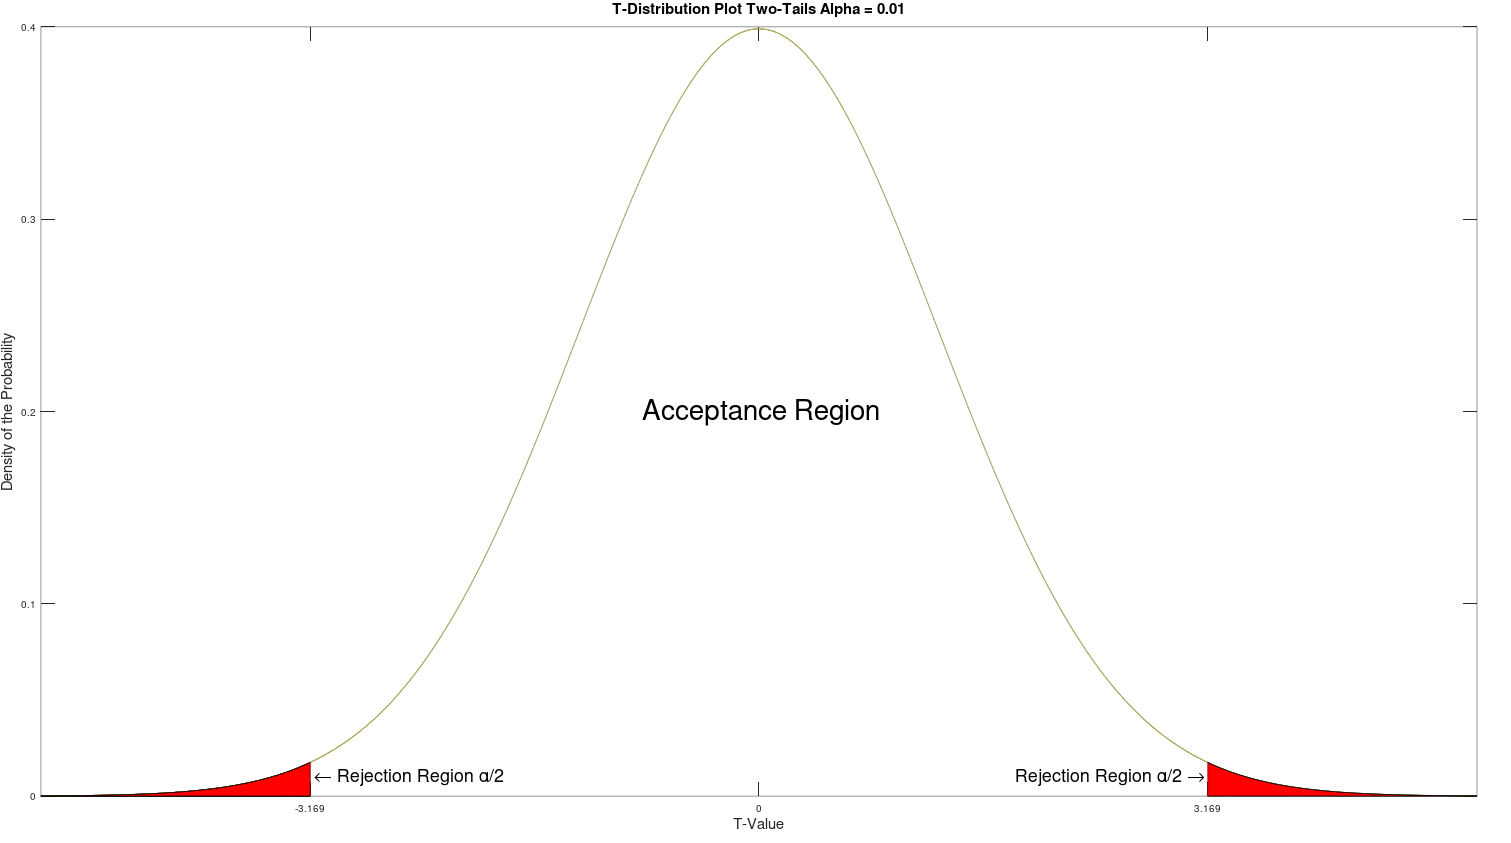
\includegraphics[scale = 0.39]{question2}\\
\hspace*{2cm}\text{Above figure shows us the acceptance and rejection regions of Question-2.}\\
\vspace*{0.2cm}\\
\section*{Answer 3}
\hspace*{-0.6cm}\text{Before we even begin solving the questions, let us define a formal representation for our given para-}\\
\text{meters in a more formal way so that it gets easier to follow along. We have 2 cases and we assume}\\
\text{that the samples are independently collected and the sample sizes are the same, n$_X$ = n$_Y$ = 68.}\\
\vspace*{0.2cm}\\
\text{Our first case, X, is the painkillers existing in the market:}\\
\hspace*{0.6cm}\text{Reduce the headache in 3 minutes, such that $\bar{X}$ = 3,}\\
\hspace*{0.6cm}\text{The standard deviation of the time required for reducing the headache is 1.4 minute, $\sigma_X$ = 1.4.}\\
\text{Our second case, Y, is the new painkiller:}\\
\hspace*{0.6cm}\text{On average reduce the headache in 2.8 minutes, such that $\bar{Y}$ = 2.8,}\\
\hspace*{0.6cm}\text{The standard deviation of the time required for reducing the headache is 1.7 minute, $\sigma_Y$ = 1.7.}\\
\vspace*{0.1cm}\\
\subsection*{a)}
\[H_0: \mu_Y = \mu_X\]\\
\subsection*{b)}
\hspace*{-0.6cm}\text{The two-sided alternative of the null hypothesis H$_A$: $\mu_y$ $\neq$ $\mu_X$. However, if we worry about longer}\\
\text{time required to reduce the headache only, we can conduct a one-sided test of:}\\
\[H_A: \mu_Y < \mu_X\]\\
\subsection*{c)}
\hspace*{-0.6cm}\text{This corresponds to a right-tailed test, for which a Z-test for two population means, with known}\\
\text{population standard deviations will be used. Based on the information provided, the significance}\\
\text{level is $\alpha$ = 0.05, and the critical value for a right-tailed test is Z$_c$ = 1.64. The rejection region for}\\
\text{this right-tailed test is:}\\
\[\mathcal{R} = [1.640, \infty) \]\\
\text{The z-statistic is computed as follows:}\\
\[z = \frac{\bar{X} - \bar{Y}}{\sqrt{\frac{\sigma_X^2}{n_X} + \frac{\sigma_Y^2}{n_Y}}}\]\\
\[\hspace*{0.6cm} = \frac{3 - 2.8}{\sqrt{\frac{1.4^2}{68} + \frac{1.7^2}{68}}}\]\\
\[\hspace*{-0.8cm} = 0.749\]\\
\text{Since it is observed that \textit{z} = 0.749 $\leq$ Z$_c$ = 1.64, calculated z value is in the '\textit{Acceptance Region}', it}\\
\text{is then concluded that there is not sufficient evidence to reject the null hypothesis. Therefore, we}\\
\text{can state that, \textbf{with 5\% significance level we do not have sufficient evidence to say the}}\\
\text{\textbf{new painkiller really produce better results}.}\\
\vspace*{0.2cm}\\
\hspace*{-2.2cm}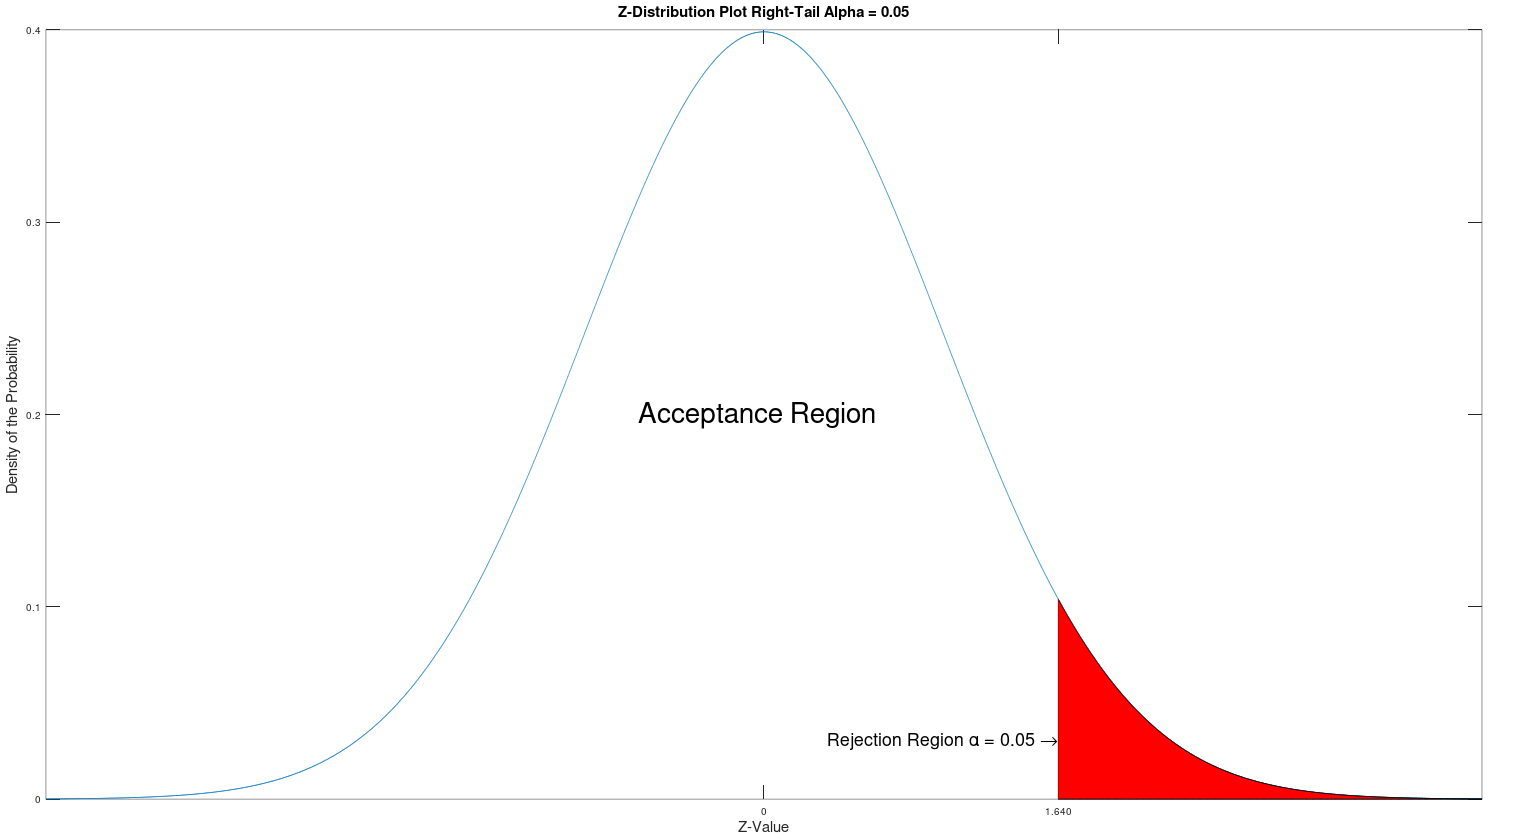
\includegraphics[scale = 0.39]{question3}\\
\hspace*{2cm}\text{Above figure shows us the acceptance and rejection region of Question-3.}\\
\end{document}


